% =============================================================================
% Second-review paper -- IEEE conference format (IEEEtran), max 6 pages.
%
% HOW TO USE THIS FILE (team):
%  * Text from our first-review proposal is kept and switched to past tense.
%  * Paragraphs marked  %%% AI-DRAFTED  were drafted by the AI assistant
%    (method details that did not exist in the proposal). Please re-read and
%    rephrase them in your own words before submission.
%  * The former red boxes are now filled with AI-drafted text (marked
%    %%% AI-DRAFTED). Rewrite them in your own words to meet the <20% AI limit.
%  * Red boxes  \teamwrite{...}{N}  (none left) marked paragraphs WE must write ourselves.
%    The facts and exact numbers to use are in the  %%% NOTES  comment above
%    each box (all numbers come from results/ in the GitHub repo).
%    Each box reserves roughly N lines so the page count stays realistic.
%    Delete the \teamwrite line once the paragraph is written.
%  * Tables in tables/ and figures in figures/ are generated by the code
%    (src/report.py); do not edit them by hand. Re-copy with
%    paper/update_from_results.sh if results change.
% =============================================================================
\documentclass[conference]{IEEEtran}
\IEEEoverridecommandlockouts
\usepackage{cite}
\usepackage{amsmath,amssymb,amsfonts}
\usepackage{graphicx}
\usepackage{booktabs}
\usepackage{xcolor}
\usepackage{url}
\usepackage[hidelinks]{hyperref}

% ---- marker for paragraphs the team writes (delete when done) ---------------
\newcommand{\teamwrite}[2]{\par\noindent\fcolorbox{red}{red!4}{\parbox[t][#2\baselineskip][t]{\dimexpr\columnwidth-2\fboxsep-2\fboxrule\relax}{\footnotesize\color{red}\textbf{TEAM TO WRITE:} #1 (about #2 lines). Facts and numbers: see the NOTES comment above this box in main.tex.}}\par\medskip}

\begin{document}

\title{Who Should We Market To? Uplift Modeling with Causal Machine Learning on a Large-Scale Randomized Advertising Experiment}

\author{\IEEEauthorblockN{Aparna Chaudhary (Team Lead), Pramit Manna, Akash Anant}
\IEEEauthorblockA{Big Data Analytics, Goa Institute of Management, Goa, India\\
Roll Numbers: B2026007, B2026031, B2026004\\
\{aparna.chaudhary2026b, pramit.manna2026b, akashanant2026b\}@gim.ac.in}}

\maketitle

\begin{abstract}
Marketing budgets are wasted when campaigns target customers who would have converted anyway, or whose behavior a campaign cannot change. This paper presents a machine learning project on uplift modeling, which estimates the incremental effect of a campaign on each customer. We used the public Criteo Uplift Prediction Dataset, a randomized advertising trial with about 14 million users, to compare a conventional response model with three uplift approaches: a two-model approach, a transformed-outcome approach and a causal forest. Models were evaluated on held-out data using Qini curves, uplift at the top-$k$ users, paired bootstrap confidence intervals and a budget simulation.
% %%% NOTES for the abstract's result sentences (2-3 sentences, write yourselves):
%  - sample: 2,000,000 users; test: 400,000 users; primary outcome visit.
%  - only the causal forest beat the response baseline on AUQC: +0.44 per 1,000
%    users, 95% CI [0.13, 0.81]; T-learner and transformed outcome did not.
%  - contacting everyone lost 444.1 per 1,000 users (V=100, c=1.5); targeting
%    ~20-24% of users gave 450-530; causal forest highest (530.1) but the paired
%    difference vs response (+69.7, CI [-3.8, 144.0]) was not significant.
%%% AI-DRAFTED from the NOTES above (rewrite in your own words):
On a random sample of 2,000,000 users, only the causal forest ranked users better than the response model, raising the area under the Qini curve by 0.44 incremental visits per 1,000 users (95\% CI 0.13 to 0.81); the two-model and transformed-outcome approaches did not beat the baseline. Under illustrative costs, contacting every user lost 444.1 per 1,000 users, while contacting the top 19--24\% ranked by any model earned between 450.0 and 530.1. The causal forest earned the most, but its advantage over the response model was not statistically significant.
\end{abstract}

\begin{IEEEkeywords}
Uplift Modeling, Causal Machine Learning, Marketing Analytics, Heterogeneous Treatment Effects, Qini Curve
\end{IEEEkeywords}

% =============================================================================
\section{Introduction}
The business problem addressed in this project was deciding which customers to target with a marketing campaign. A standard response model ranks customers by their probability of buying. That probability is high for customers who would have bought without any contact, so spending is concentrated on the wrong people. The question that matters for a marketing manager is causal: for which customers does contacting them \emph{increase} the chance of a desired outcome? Answering it can improve return on marketing spend, reduce unnecessary contacts and support better decisions in advertising, retail, banking and telecommunications.

\subsection{Scope and Objectives}
The project compared methods for ranking customers by their estimated incremental response, and translated ranking quality into a budget decision, using real data from a randomized experiment. The objectives were:
\begin{itemize}
\item Establishing the relevance of incremental (uplift) targeting versus response-based targeting.
\item Demonstrating originality through a like-for-like comparison of four methods with uncertainty estimates.
\item Evaluating with metrics suited to causal problems (Qini curves and uplift at top-$k$) rather than accuracy.
\item Converting model rankings into a profit-based targeting decision under stated cost assumptions.
\item Ensuring reproducibility and transparency in data and methods.
\end{itemize}

% =============================================================================
\section{Related Work}
Uplift modeling, also called incremental response modeling, was formalized for direct marketing by Radcliffe~\cite{radcliffe2007}, who stressed the use of control groups to target on predicted lift. Tree-based uplift methods modify the splitting criterion to maximize treatment-effect differences~\cite{rzepakowski2012}. The class-transformation approach~\cite{jaskowski2012} and the transformed-outcome idea~\cite{athey2016} reduce uplift estimation to a single supervised learning problem. Meta-learners such as the two-model approach are analyzed by K\"unzel et al.~\cite{kunzel2019}, and forest-based estimators give flexible non-parametric treatment-effect estimates~\cite{wager2018,athey2019}. Gutierrez and G\'erardy~\cite{gutierrez2017} review the literature, and Diemert et al.~\cite{diemert2018} released the large-scale Criteo benchmark that we used.

Previous studies, such as~\cite{kunzel2019,diemert2018}, compare uplift estimators and report ranking metrics. Our approach built on these works by comparing four methods on the same large randomized sample, quantifying the uncertainty of each comparison with a paired bootstrap, and adding a decision-oriented profit evaluation in which the targeting fraction was chosen on validation data. The intended contribution is an end-to-end, reproducible comparison with a business decision layer, not a new algorithm.

% =============================================================================
\section{Methodology}
This section describes the data, preprocessing, models and evaluation metrics.

\subsection{Data}
We used the Criteo Uplift Prediction Dataset (v2.1)~\cite{diemert2018,criteo}, collected from an incrementality test in which a random subset of users was not targeted by advertising. It contains 13,979,592 users, each with 12 anonymized numerical features, a binary treatment indicator (85\% treated), the outcomes \emph{visit} and \emph{conversion}, and an \emph{exposure} indicator. The data is publicly available from the Criteo AI Lab page.
%%% AI-DRAFTED (rephrase):
Because the official download link redirected to a storage server that was unreachable during the project, we downloaded a public copy of the same file and verified that its SHA-256 checksum matched the checksum of the official file.

Preprocessing included drawing a simple random sample of the data (which preserves the randomization of treatment), using the randomized treatment indicator rather than exposure, a stratified train/validation/test split, and a randomization check comparing feature distributions between treated and control users.
%%% AI-DRAFTED (rephrase):
The sample contained 2,000,000 users (seed 42), split 60/20/20 into training (1.2M), validation (0.4M) and test (0.4M) sets, stratified by treatment $\times$ visit. The primary outcome was \emph{visit}; \emph{conversion} (about 0.3\% of users) was treated as a secondary outcome because it is too rare for precise comparisons. Table~\ref{tab:profile} profiles the full file and the sample, and Table~\ref{tab:rand} reports standardized mean differences (SMD) between treated and control users.

\begin{table}[t]
\centering
\caption{Dataset profile (full file and the 2M-user sample)}
\label{tab:profile}
\footnotesize
% Auto-generated by src/report.py from results/*.csv -- do not edit by hand.
\begin{tabular}{lrr}
\toprule
 & Full file & Sample \\
\midrule
Users & 13,979,592 & 2,000,000 \\
Treated share (\%) & 85.00 & 85.04 \\
Visit rate, treated (\%) & 4.854 & 4.862 \\
Visit rate, control (\%) & 3.820 & 3.807 \\
Visit ATE (pp) & 1.034 & 1.056 \\
Conversion rate, treated (\%) & 0.309 & 0.316 \\
Conversion rate, control (\%) & 0.194 & 0.193 \\
Conversion ATE (pp) & 0.115 & 0.124 \\
Exposure rate, treated (\%) & 3.60 & 3.59 \\
\midrule
Train / valid / test & & 1,200,000 / 400,000 / 400,000 \\
\bottomrule
\end{tabular}

\end{table}

\begin{table}[t]
\centering
\caption{Randomization check: feature means and standardized mean differences (treated vs.\ control)}
\label{tab:rand}
\footnotesize
% Auto-generated by src/report.py from results/*.csv -- do not edit by hand.
\begin{tabular}{lrrrrr}
\toprule
Feature & Mean (T) & Mean (C) & SMD & SMD (full) & $z$ (full) \\
\midrule
f0 & 19.618 & 19.651 & $-$0.0062 & $-$0.0069 & $-$9.2 \\
f1 & 10.070 & 10.068 & +0.0267 & +0.0240 & +33.7 \\
f2 & 8.446 & 8.449 & $-$0.0086 & $-$0.0062 & $-$8.3 \\
f3 & 4.170 & 4.235 & $-$0.0495 & $-$0.0488 & $-$67.2 \\
f4 & 10.339 & 10.336 & +0.0087 & +0.0080 & +10.7 \\
f5 & 4.027 & 4.039 & $-$0.0303 & $-$0.0306 & $-$42.3 \\
f6 & $-$4.183 & $-$3.989 & $-$0.0428 & $-$0.0404 & $-$54.7 \\
f7 & 5.105 & 5.083 & +0.0187 & +0.0213 & +28.8 \\
f8 & 3.933 & 3.935 & $-$0.0221 & $-$0.0224 & $-$30.2 \\
f9 & 16.044 & 15.888 & +0.0226 & +0.0240 & +32.5 \\
f10 & 5.334 & 5.332 & +0.0094 & +0.0106 & +14.2 \\
f11 & $-$0.171 & $-$0.171 & $-$0.0058 & $-$0.0052 & $-$6.9 \\
\midrule
\multicolumn{6}{l}{SD of SMD expected under randomization (full file): 0.0007} \\
\multicolumn{6}{l}{Classifier AUC, treatment from features (test): 0.5103 [0.5079, 0.5130]} \\
\bottomrule
\end{tabular}

\end{table}

\subsection{Models and Techniques}
Let $Y$ be the outcome, $T \in \{0,1\}$ the treatment and $X$ the features. The target quantity is the conditional average treatment effect
\begin{equation}
\tau(x) = \mathbb{E}[Y(1) - Y(0) \mid X = x],
\end{equation}
which is never observed for an individual user. We compared four scoring methods:
\begin{itemize}
\item \textbf{Response model (baseline):} predicts the probability of the outcome while ignoring treatment.
\item \textbf{Two-model approach (T-learner):} fits separate models on treated and control users and scores their difference~\cite{kunzel2019}.
\item \textbf{Transformed outcome:} learns a transformed outcome whose expectation equals $\tau(x)$ under randomization~\cite{jaskowski2012,athey2016}.
\item \textbf{Causal forest:} a forest-based estimator of heterogeneous effects~\cite{wager2018,athey2019}, implemented with EconML~\cite{econml}.
\end{itemize}
The rationale for model selection was to cover the main families of uplift estimators: a non-causal baseline, a simple meta-learner, a direct transformation and a forest designed for heterogeneous effects.

%%% AI-DRAFTED (rephrase):
Because only 15\% of users were in the control group, the class-transformation approach of~\cite{jaskowski2012}, which assumes equal group sizes, was replaced by the propensity-weighted transformed outcome of~\cite{athey2016}, $Z = YT/p - Y(1-T)/(1-p)$, with $p$ the treated share in the training set ($p = 0.8504$). The first three methods used LightGBM~\cite{lightgbm} gradient-boosted trees (learning rate 0.05, 31 leaves, at least 500 users per leaf; 0.02 and 2,000 for the transformed outcome) with early stopping on the validation set. The causal forest (\texttt{CausalForestDML}, 200 trees, at least 200 users per leaf) was trained on a random subsample of 200,000 training users to keep the run under 20 minutes on a free Colab machine; its outcome model was LightGBM and, since treatment was randomized, its propensity model was the constant treated share~\cite{chernozhukov2018}.

\subsection{Evaluation Metrics}
Because individual effects cannot be observed, models were evaluated on groups. Users in the held-out test set were sorted by predicted score, and the Qini curve gives the cumulative incremental outcomes among the top $k$ users:
\begin{equation}
Q(k) = Y_k^T - Y_k^C \frac{N_k^T}{N_k^C},
\end{equation}
where $Y_k^T, Y_k^C$ are outcomes among treated and control users in the top $k$, and $N_k^T, N_k^C$ their counts. We report the Qini coefficient (AUQC, the area between the model curve and random targeting, with both axes divided by $N$ and reported per 1,000 users), observed uplift among the top 10\%, 20\% and 30\% of users, and bootstrap confidence intervals, including paired differences against the baseline. These metrics use only observed outcomes and treatment assignment, and they directly measure whether a ranking places responsive users first.
%%% AI-DRAFTED (rephrase):
Confidence intervals are percentile intervals from 200 bootstrap resamples of test users; the same resamples were used for every method, so differences between methods are paired.

\subsection{Budget Simulation}
The profit per 1,000 users from contacting a fraction $\phi$ of users is
\begin{equation}
\Pi(\phi) = 1000 \left( V \frac{U(\phi N)}{N} - c\,\phi \right),
\end{equation}
where $V$ is the value of an incremental outcome and $c$ the cost per contact. Both are illustrative assumptions that were stated explicitly and varied in a sensitivity analysis.
%%% AI-DRAFTED (rephrase):
Here $U(k) = Q(k)\,k/N_k^T = k(\bar{y}_k^T - \bar{y}_k^C)$ is the number of incremental visits if all top-$k$ users are contacted; we used it instead of $Q(k)$ because, with 85\% treated users, $Q(k)$ counts incremental outcomes only on the treated scale. The main scenario used $V = 100$ per incremental visit and $c = 1.5$ per contact; the grid used $V \in \{50, 100, 200\}$ and $c \in \{0.5, 1, 1.5, 2, 3\}$.
The targeting fraction was chosen on the validation split (grid of 1\% steps) and evaluated on the test split.

% =============================================================================
\section{Results}

% %%% NOTES -- Data and randomization (Tables I-II):
%  - Full file 13,979,592 users, 85.00% treated; sample 2,000,000, 85.04% treated.
%  - Visit rate treated 4.862% vs control 3.807% (sample); ATE = 1.056 pp,
%    95% CI [0.980, 1.131]; relative lift 27.7%. Full file: ATE 1.034 pp [1.006, 1.063].
%  - Conversion: 0.316% vs 0.193%; ATE 0.124 pp [0.106, 0.141] (sample);
%    relative lift 64%.
%  - Only 3.59% of treated users were actually exposed to an ad -> the effects
%    are intention-to-treat effects of being *targetable*, which is why they are small.
%  - Splits: treated share 85.04% and visit rate 4.704% in all three splits
%    (stratification worked).
%  - All |SMD| < 0.05 (largest: f3 = -0.0495, f6 = -0.0428, f5 = -0.0303),
%    well below the usual 0.1 threshold. BUT be honest: with 14M users these
%    differences are far larger than random noise (SE of an SMD here is about
%    0.002) and they also appear in the full file (f3 -0.0488), so the groups
%    are not perfectly identical in the published data -- probably a feature of
%    how the dataset was built. The differences are small in size.
%%% AI-DRAFTED from the NOTES above (rewrite in your own words):
Table~\ref{tab:profile} shows that the sample closely matched the full file. In the sample, 85.04\% of users were treated, and the visit rate was 4.862\% for treated users against 3.807\% for control users. Being in the treated group therefore raised the visit rate by 1.056 percentage points (pp) (95\% CI 0.980 to 1.131), a relative lift of 27.7\%. Conversion was much rarer (0.316\% against 0.193\%, an effect of 0.124 pp). Only 3.59\% of treated users were actually shown an ad, so these are effects of being eligible for targeting, which is why they are small. The stratified split kept the treated share (85.04\%) and the visit rate (4.704\%) the same in all three parts. In Table~\ref{tab:rand}, every standardized mean difference was below 0.05 in absolute value, well under the common threshold of 0.1; the largest were for f3 ($-0.0495$) and f6 ($-0.0428$). These gaps are small, but with this many users they are larger than chance alone would produce, and they also appear in the full file, so the published groups are not perfectly balanced.

\begin{table*}[t]
\centering
\caption{Ranking quality on the test set (400,000 users). Estimates with 95\% bootstrap CIs (200 paired resamples). $\Delta$ rows: paired difference to the response model.}
\label{tab:main}
\footnotesize
% Auto-generated by src/report.py from results/*.csv -- do not edit by hand.
\begin{tabular}{lcccc}
\toprule
Method & AUQC ($\times10^3$) & Top 10\% uplift (pp) & Top 20\% uplift (pp) & Top 30\% uplift (pp) \\
\midrule
\multicolumn{5}{l}{\textit{Estimates (test ATE 1.059 pp)}} \\
Response & 3.073 [2.480, 3.632] & 4.66 [3.24, 5.94] & 3.89 [3.13, 4.64] & 3.00 [2.45, 3.52] \\
T-learner & 3.098 [2.516, 3.769] & 5.71 [4.51, 6.93] & 3.96 [3.24, 4.68] & 2.96 [2.49, 3.46] \\
X-learner & 3.539 [2.932, 4.096] & 6.25 [5.16, 7.43] & 4.43 [3.73, 5.14] & 3.17 [2.67, 3.65] \\
Transf. outcome & 3.366 [2.781, 3.949] & 6.65 [5.41, 7.80] & 4.06 [3.36, 4.73] & 2.99 [2.53, 3.48] \\
DR-learner & 3.071 [2.486, 3.683] & 6.14 [4.90, 7.33] & 3.76 [3.02, 4.53] & 2.89 [2.36, 3.41] \\
Causal forest & 3.200 [2.603, 3.789] & 5.86 [4.58, 7.05] & 3.86 [3.10, 4.64] & 2.90 [2.35, 3.41] \\
Hybrid & 3.539 [2.932, 4.096] & 6.25 [5.16, 7.43] & 4.43 [3.73, 5.14] & 3.17 [2.67, 3.65] \\
\midrule
\multicolumn{5}{l}{\textit{Paired difference to the response model ($^{*}$: significant after Holm correction over all 24 comparisons)}} \\
T-learner & +0.025 [$-$0.529, 0.677] & +1.05 [0.12, 1.93] & +0.06 [$-$0.37, 0.51] & $-$0.03 [$-$0.32, 0.30] \\
X-learner & +0.466 [$-$0.073, 0.965] & +1.59 [0.73, 2.49]$^{*}$ & +0.54 [0.11, 0.93] & +0.17 [$-$0.09, 0.44] \\
Transf. outcome & +0.293 [$-$0.201, 0.819] & +1.99 [1.00, 2.85]$^{*}$ & +0.16 [$-$0.24, 0.62] & +0.00 [$-$0.24, 0.27] \\
DR-learner & $-$0.002 [$-$0.333, 0.307] & +1.48 [0.53, 2.38] & $-$0.13 [$-$0.45, 0.21] & $-$0.11 [$-$0.29, 0.10] \\
Causal forest & +0.127 [0.003, 0.252] & +1.19 [0.48, 1.85]$^{*}$ & $-$0.03 [$-$0.29, 0.25] & $-$0.10 [$-$0.23, 0.05] \\
Hybrid & +0.466 [$-$0.073, 0.965] & +1.59 [0.73, 2.49]$^{*}$ & +0.54 [0.11, 0.93] & +0.17 [$-$0.09, 0.44] \\
\bottomrule
\end{tabular}

\end{table*}

\begin{figure}[t]
\centering
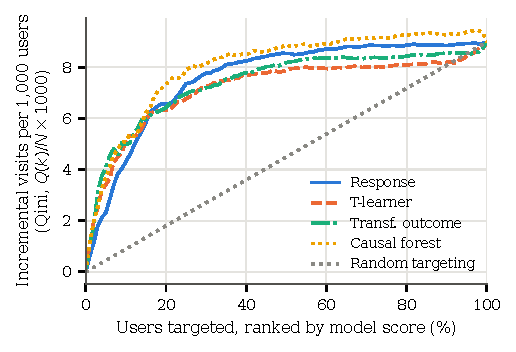
\includegraphics[width=\columnwidth]{figures/qini_curves_visit.pdf}
\caption{Qini curves for visit on the test set, compared with random targeting.}
\label{fig:qini}
\end{figure}

\begin{figure}[t]
\centering
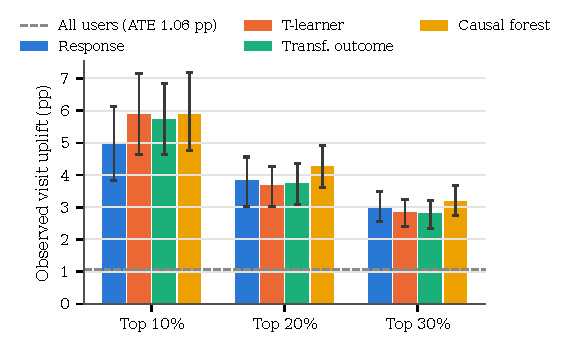
\includegraphics[width=\columnwidth]{figures/uplift_topk_visit.pdf}
\caption{Observed visit uplift among the top 10/20/30\% of test users ranked by each model, with 95\% bootstrap CIs. Dashed: average effect over all users.}
\label{fig:topk}
\end{figure}

% %%% NOTES -- Ranking quality for VISIT (Table III, Figs. 1-2):
%  - Test ATE (visit) = 1.056 pp, bootstrap 95% CI [0.892, 1.204].
%  - AUQC (x10^3, per 1,000 users): Response 3.090 [2.559, 3.648];
%    T-learner 2.679 [2.095, 3.287]; Transf. outcome 2.898 [2.338, 3.535];
%    Causal forest 3.531 [3.030, 4.086].
%  - Paired AUQC differences vs response: T-learner -0.411 [-0.987, 0.231];
%    Transf. outcome -0.192 [-0.848, 0.428]; Causal forest +0.440 [0.127, 0.814]
%    -> ONLY the causal forest is significantly better (0 of 200 bootstrap
%    differences <= 0). The two simpler uplift models were NOT better than the
%    response model overall (point estimates are lower, CIs include 0).
%  - Top 10%: Response 4.99 pp; T-learner 5.89; Transf. outcome 5.73;
%    Causal forest 5.89. Differences vs response: T-learner +0.90 [0.06, 1.94]
%    (significant), Transf. outcome +0.74 [-0.23, 1.74], CF +0.90 [-0.09, 1.74].
%    Top-10% users have about 5-6x the average uplift (5.89 / 1.056 = 5.6x).
%  - Top 20%: Response 3.82; T 3.68; TO 3.73; CF 4.27; CF diff +0.45 [0.04, 0.84]
%    (significant).
%  - Top 30%: Response 3.03; T 2.83; TO 2.81; CF 3.18; all differences include 0.
%  - Qini curve (Fig. 1), incremental visits per 1,000 users captured
%    (total over all users = 8.98):
%      at 10% targeted: Resp 4.31, T 5.09, TO 4.97, CF 5.10
%      at 20%:          Resp 6.55, T 6.31, TO 6.41, CF 7.32
%      at 50%:          Resp 8.54, T 7.89, TO 8.18, CF 8.87
%    -> T-learner/TO help only for the first ~15% of users; after that the
%    response model ranks better; CF is at or above the others almost everywhere.
%  - All models are far above random targeting.
%  - Spearman rank correlation of test scores (results/score_correlations.csv):
%    response vs CF 0.675, response vs TO 0.696, response vs T 0.599 ->
%    the response model's ranking overlaps strongly with the uplift rankings,
%    i.e. users likely to visit are also those whose visits the ad increases most.
%%% AI-DRAFTED from the NOTES above (rewrite in your own words):
Table~\ref{tab:main} and Fig.~\ref{fig:qini} give the main comparison. All four models were far better than random targeting, and the response model proved a strong baseline, with an AUQC of 3.090 per 1,000 users. The causal forest reached 3.531, and its paired difference of 0.440 (95\% CI 0.127 to 0.814) was the only AUQC gain whose interval excluded zero. The T-learner (2.679) and the transformed-outcome model (2.898) scored below the baseline, although their intervals for the difference included zero.

The picture changed at the very top of the ranking (Fig.~\ref{fig:topk}). Among the top 10\% of users, the observed visit uplift was 4.99~pp for the response model and 5.89~pp for both the T-learner and the causal forest, more than five times the average effect of 1.056~pp. Only the T-learner's gain here was significant (0.90~pp, CI 0.06 to 1.94). Beyond about 15\% of users, the Qini curves of the T-learner and the transformed-outcome model fell below that of the response model: at 50\% targeted they captured 7.89 and 8.18 incremental visits per 1,000 users, against 8.54 for the response model and 8.87 for the causal forest. The causal forest was also significantly better in the top 20\% (4.27 against 3.82~pp; difference 0.45, CI 0.04 to 0.84).

% %%% NOTES -- CONVERSION (secondary), Table III lower panel:
%  - Test ATE 0.109 pp (CI [0.062, 0.145]); only 1,201 conversions in the test
%    set, of which 124 in the control group (59,847 control users).
%  - AUQC x10^3: Response 0.362, T 0.272, TO 0.324, CF 0.363.
%  - No paired difference vs response is significant (all CIs include 0;
%    e.g. CF +0.001 [-0.040, 0.058]). Conclusion: conversion is too rare in a
%    2M sample to separate the methods -- as expected in the proposal.
%%% AI-DRAFTED from the NOTES above (rewrite in your own words):
For conversion, the average effect on the test set was only 0.109~pp, and the test control group contained just 124 conversions. AUQC values ranged from 0.272 (T-learner) to 0.363 (causal forest), and none of the differences from the response model was significant. As anticipated in the proposal, conversion was too rare in this sample to separate the methods.

\begin{figure}[t]
\centering
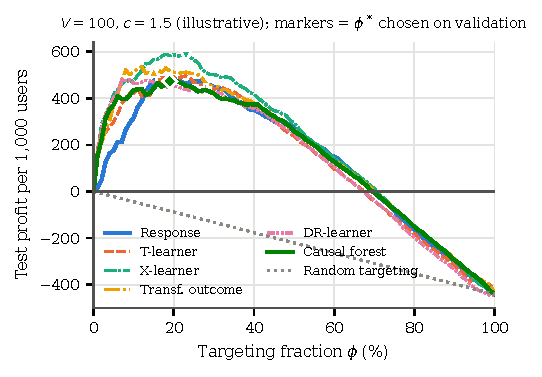
\includegraphics[width=\columnwidth]{figures/profit_vs_targeting_fraction.pdf}
\caption{Test-set profit per 1,000 users against the targeting fraction ($V=100$, $c=1.5$, illustrative). Markers: fraction $\phi^*$ chosen on the validation set.}
\label{fig:profit}
\end{figure}

\begin{table}[t]
\centering
\caption{Budget simulation, $V=100$, $c=1.5$ (illustrative). $\phi^*$ chosen on validation; profit per 1,000 test users. Oracle: best $\phi$ on test (not achievable).}
\label{tab:budget}
\setlength{\tabcolsep}{3pt}
\scriptsize
% Auto-generated by src/report.py from results/*.csv -- do not edit by hand.
\begin{tabular}{lrlll}
\toprule
Policy & $\phi^*$ & Test profit [95\% CI] & $\Delta$ vs Resp. [95\% CI] & Oracle ($\phi$) \\
\midrule
Contact nobody & 0\% & 0.0 & -- & -- \\
Contact everyone & 100\% & $-$441.1 & -- & -- \\
Random targeting & 0\% & 0.0 & -- & -- \\
Response & 20\% & 478.9 [325.1, 630.7] & -- & 496.8 (18\%) \\
T-learner & 17\% & 476.8 [335.9, 611.7] & $-$2.1 [$-$91.1, 86.3] & 496.0 (23\%) \\
X-learner & 23\% & 581.6 [432.2, 725.1] & +102.7 [14.0, 185.6] & 588.8 (18\%) \\
Transf. outcome & 15\% & 513.8 [361.8, 643.7] & +34.9 [$-$61.9, 127.7] & 536.3 (12\%) \\
DR-learner & 28\% & 439.5 [279.6, 596.4] & $-$39.3 [$-$104.3, 25.1] & 480.4 (7\%) \\
Causal forest & 19\% & 472.4 [313.0, 626.5] & $-$6.4 [$-$64.0, 42.5] & 472.4 (19\%) \\
Hybrid & 23\% & 581.6 [432.2, 725.1] & +102.7 [14.0, 185.6] & 588.8 (18\%) \\
\bottomrule
\end{tabular}

\end{table}

% %%% NOTES -- Budget simulation (Table IV, Fig. 3), V=100, c=1.5:
%  - Contacting everyone: -444.1 per 1,000 users, because the average uplift
%    (1.056 pp) is below the break-even uplift c/V = 1.5 pp.
%    Random targeting therefore chose phi = 0 (profit 0).
%  - phi* chosen on validation: Response 23%, T 19%, TO 21%, CF 24%.
%  - Test profit per 1,000 users [95% CI]: Response 460.4 [289.0, 622.4];
%    T-learner 450.0 [310.2, 601.4]; Transf. outcome 454.9 [320.2, 591.5];
%    Causal forest 530.1 [391.9, 690.0].
%  - Paired difference vs response: T -10.5 [-95.1, 68.1]; TO -5.6 [-101.3, 74.0];
%    CF +69.7 [-3.8, 144.0] (97% of bootstrap differences > 0, but the CI
%    includes 0 -> not significant at 5%).
%  - Oracle (best phi on test): Response 488.3 at 16%, T 480.9 at 16%,
%    TO 479.4 at 14%, CF 565.6 at 21% -> choosing phi on validation cost only
%    24.5-35.5 per 1,000 users vs the oracle; the validation rule worked.
%  - Swing from "contact everyone" to model targeting: 894-974 per 1,000 users.
% %%% NOTES -- Sensitivity grid (results/sensitivity_grid.csv, 15 (V,c) pairs):
%  - Best model per scenario: causal forest 9/15, transformed outcome 4/15
%    (high cost relative to value: c/V >= 0.03), response 2/15 (c/V = 0.02,
%    margins of 1.1 and 2.2 per 1,000).
%  - Profit depends only on c/V up to scale (e.g. (50,1) and (100,2) give the same phi*).
%  - Contact-everyone is profitable only when c/V < 1.06% (ATE); even then the
%    best model beat it in all 15 scenarios (e.g. V=200, c=0.5: CF 1810.4 vs 1611.7).
%  - Label these numbers as illustrative.
%%% AI-DRAFTED from the NOTES above (rewrite in your own words):
With $V=100$ and $c=1.5$, contacting everyone lost 444.1 per 1,000 users, because the average uplift of 1.056~pp was below the break-even uplift of $c/V = 1.5$~pp (Table~\ref{tab:budget}); for the same reason, random targeting chose to contact nobody. The models picked targeting fractions between 19\% and 24\% on the validation set and earned between 450.0 and 530.1 per 1,000 users on the test set (Fig.~\ref{fig:profit}). The causal forest earned the most, 69.7 more than the response model, but the paired interval for this difference ($-3.8$ to 144.0) included zero. Choosing $\phi$ on validation cost between 24.5 and 35.5 per 1,000 users compared with the best fraction on the test set, so the rule held up on new data.

In the sensitivity grid of 15 $(V, c)$ pairs, the causal forest gave the highest profit in 9, the transformed-outcome model in 4 (all with high cost relative to value, $c/V \ge 0.03$) and the response model in 2, by margins of at most 2.2. The best model beat contacting everyone in all 15 cases. These figures depend on the assumed values and are illustrative only.

% =============================================================================
\section{Discussion, Originality and Limitations}

% %%% NOTES -- Discussion (write in your own words):
%  - Main answer to "who should we market to?": rank users by estimated uplift
%    and contact only the top ~20-25% under these costs; blanket contact loses money.
%  - Honest finding: the response model was a strong baseline on this data.
%    Two of three uplift methods did NOT beat it overall; only the causal forest
%    improved AUQC significantly (+0.44 per 1,000 users, about +14%).
%  - Likely reasons (present as explanations, not proven):
%     * response score and uplift are positively related here (rank corr. 0.60-0.70);
%     * the control group is small: 179,540 control users in training with
%       only 6,835 visits, so the control-side model / transformed outcome is noisy;
%     * the transformed outcome Z takes values -6.68, 0 and +1.18 -> very high
%       variance; early stopping kept only 141 trees;
%     * the causal forest targets tau(x) directly with honest splitting, even on
%       only 200k users.
%  - Business: the difference between methods (tens per 1,000 users) is small
%    compared with the difference between targeting and not targeting (~900).
%  - Comparison with benchmark [9] (Diemert et al.): check their paper for what
%    they report on visit before writing any comparison -- do not guess numbers.
%  - Originality: four estimators on one randomized sample, paired bootstrap
%    CIs, validation-based phi rule, and a fully reproducible repo.
%%% AI-DRAFTED from the NOTES above (rewrite in your own words):
The answer to our title question is to rank users by estimated uplift and contact only about the top fifth; under our cost assumptions a blanket campaign lost money. The less expected finding is how well the response model did. Two of the three uplift methods did not beat it overall, and only the causal forest improved AUQC significantly, by about 14\%.

We see three likely reasons, which we did not test directly. First, on this data the response score and the uplift scores were closely related (rank correlations between 0.60 and 0.70), so users likely to visit were also those whose visits the ad raised most. Second, the control group was small: the training set had 179,540 control users with only 6,835 visits, which makes the control-side model of the T-learner noisy. Third, the transformed outcome takes only the values $-6.68$, 0 and $+1.18$, so its target is very noisy, and early stopping kept only 141 trees. The causal forest estimates the effect directly, which may explain why it did better even when trained on only 200,000 users.

For a manager, the gap between methods (tens per 1,000 users) mattered far less than the gap between targeting and not targeting (894 to 974 per 1,000 users). The originality of the study lies in comparing four estimators on one randomized sample with paired intervals, choosing the targeting fraction on separate data, and publishing everything needed to repeat the analysis.

We anticipated the following limitations, and they applied. Uplift effects were small relative to outcome noise, so estimates were uncertain. The anonymized features prevented interpreting which customer traits drive response. The analysis used treatment assignment, not whether an ad was actually seen. Sampling and subsampling were needed for computational reasons. The value and cost parameters were illustrative, and the results come from one advertising experiment and may not transfer to other industries.
% %%% NOTES -- extra limitations to add in your own words:
%  - only 3.6% of treated users were exposed -> intention-to-treat effects;
%  - small but systematic feature imbalance (max |SMD| 0.05, Table II);
%  - hyperparameters were fixed, not tuned; causal forest used 200k of 1.2M rows;
%  - bootstrap CIs cover test-set sampling only, not re-training variability;
%  - one 2M sample, one seed.
%%% AI-DRAFTED from the NOTES above (rewrite in your own words):
In addition, only 3.6\% of treated users were exposed, so all effects are intention-to-treat effects, and the groups showed small feature differences (Table~\ref{tab:rand}). Hyperparameters were fixed rather than tuned, and the causal forest used 200,000 of the 1.2 million training users. Finally, the bootstrap captured test-set sampling but not the variability from retraining the models, and the analysis used one sample and one seed.

% =============================================================================
\section{Reproducibility}
%%% AI-DRAFTED (rephrase):
All code, the configuration, a step-by-step Google Colab notebook and every result reported here are available at \url{https://github.com/Akash-420bit/uplift-criteo}. The README lists the exact package versions, the expected runtime and how each table and figure maps to a file in the \texttt{results/} folder. The pipeline downloads the data, verifies its checksum, and fixes all random seeds in \texttt{config.yaml}; re-running it reproduced identical model scores. The raw data is not redistributed.

\subsection{AI Use Declaration}
%%% Please check this text matches what you actually did, then keep it.
%%% TEAM: update this to say which parts you rewrote yourselves, and add the
%%% sentence about the <20% AI-content limit only if it is true after your edits.
An AI assistant (Claude, by Anthropic) was used in two phases. For the first-review proposal it helped develop the project idea and draft the wording. For this paper it wrote the analysis code (data preparation, models, evaluation, bootstrap and budget simulation), tested it on synthetic data, ran it on the Criteo data, generated the tables and figures from the code's output, converted the proposal text to the IEEE template and past tense, and drafted the method details and the Results, Discussion and Conclusion text from the numbers in the results files. The authors reviewed and edited all content, checked every number against the results files in the repository, and take responsibility for the paper.

% =============================================================================
\section{Conclusion}
% %%% NOTES -- Conclusion (write yourselves, 4-6 sentences):
%  - Restate question; what was done (4 methods, 2M-user sample of the Criteo trial).
%  - Key result: targeting the top ~20-25% by any model turned a loss of 444 into a
%    profit of 450-530 per 1,000 users (illustrative costs); causal forest gave the
%    best ranking (only significant AUQC gain), simple uplift models did not beat
%    the response model overall.
%  - Next steps before the final submission: e.g. tune hyperparameters, train the
%    causal forest on more data, try X-/DR-learners, repeat with several seeds.
%%% AI-DRAFTED from the NOTES above (rewrite in your own words):
This paper asked which customers a campaign should target, using a randomized advertising trial of about 14 million users. We compared a response model with three uplift methods on a 2,000,000-user sample. Targeting the top 19--24\% of users by any model turned a loss of 444.1 per 1,000 users into a profit of 450.0 to 530.1 under illustrative costs. The causal forest gave the best ranking and was the only method with a significant AUQC gain, while the simpler uplift methods did not beat the response model overall. Before the final submission we plan to tune hyperparameters, train the causal forest on more data, add X- and doubly robust learners, and repeat the analysis with several seeds.

% =============================================================================
\begin{thebibliography}{99}
\footnotesize
\bibitem{radcliffe2007} N. J. Radcliffe, ``Using control groups to target on predicted lift: Building and assessing uplift models,'' \emph{Direct Marketing Analytics Journal}, Direct Marketing Association, pp. 14--21, 2007.
\bibitem{rzepakowski2012} P. Rzepakowski and S. Jaroszewicz, ``Decision trees for uplift modeling with single and multiple treatments,'' \emph{Knowledge and Information Systems}, vol. 32, no. 2, pp. 303--327, 2012.
\bibitem{jaskowski2012} M. Jaskowski and S. Jaroszewicz, ``Uplift modeling for clinical trial data,'' in \emph{ICML 2012 Workshop on Clinical Data Analysis}, 2012.
\bibitem{athey2016} S. Athey and G. Imbens, ``Recursive partitioning for heterogeneous causal effects,'' \emph{Proc. Natl. Acad. Sci. USA}, vol. 113, no. 27, pp. 7353--7360, 2016.
\bibitem{gutierrez2017} P. Gutierrez and J.-Y. G\'erardy, ``Causal inference and uplift modelling: A review of the literature,'' in \emph{Proc. Int. Conf. on Predictive Applications and APIs}, PMLR vol. 67, pp. 1--13, 2017.
\bibitem{kunzel2019} S. R. K\"unzel, J. S. Sekhon, P. J. Bickel, and B. Yu, ``Metalearners for estimating heterogeneous treatment effects using machine learning,'' \emph{Proc. Natl. Acad. Sci. USA}, vol. 116, no. 10, pp. 4156--4165, 2019.
\bibitem{wager2018} S. Wager and S. Athey, ``Estimation and inference of heterogeneous treatment effects using random forests,'' \emph{J. Amer. Statist. Assoc.}, vol. 113, no. 523, pp. 1228--1242, 2018.
\bibitem{athey2019} S. Athey, J. Tibshirani, and S. Wager, ``Generalized random forests,'' \emph{Ann. Statist.}, vol. 47, no. 2, pp. 1148--1178, 2019.
\bibitem{diemert2018} E. Diemert, A. Betlei, C. Renaudin, and M.-R. Amini, ``A large scale benchmark for uplift modeling,'' in \emph{Proc. AdKDD and TargetAd Workshop, KDD}, London, UK, 2018.
\bibitem{criteo} Criteo AI Lab, ``Criteo Uplift Prediction Dataset.'' [Online]. Available: \url{https://ailab.criteo.com/criteo-uplift-prediction-dataset/}
\bibitem{econml} Microsoft Research, ``EconML: A Python package for ML-based heterogeneous treatment effects estimation.'' [Online]. Available: \url{https://github.com/py-why/EconML}
\bibitem{lightgbm} G. Ke, Q. Meng, T. Finley, T. Wang, W. Chen, W. Ma, Q. Ye, and T.-Y. Liu, ``LightGBM: A highly efficient gradient boosting decision tree,'' in \emph{Advances in Neural Information Processing Systems 30}, 2017, pp. 3146--3154.
\bibitem{chernozhukov2018} V. Chernozhukov, D. Chetverikov, M. Demirer, E. Duflo, C. Hansen, W. Newey, and J. Robins, ``Double/debiased machine learning for treatment and structural parameters,'' \emph{The Econometrics Journal}, vol. 21, no. 1, pp. C1--C68, 2018.
\end{thebibliography}

\end{document}
